\documentclass[tikz]{standalone}
\usepackage{tkz-graph}
\usepackage{amsmath,amssymb}
\usepackage{xcolor}
\usetikzlibrary{calc}
\usetikzlibrary{positioning}

\begin{document}

% https://latexdraw.com/exploring-tikz-arrows/
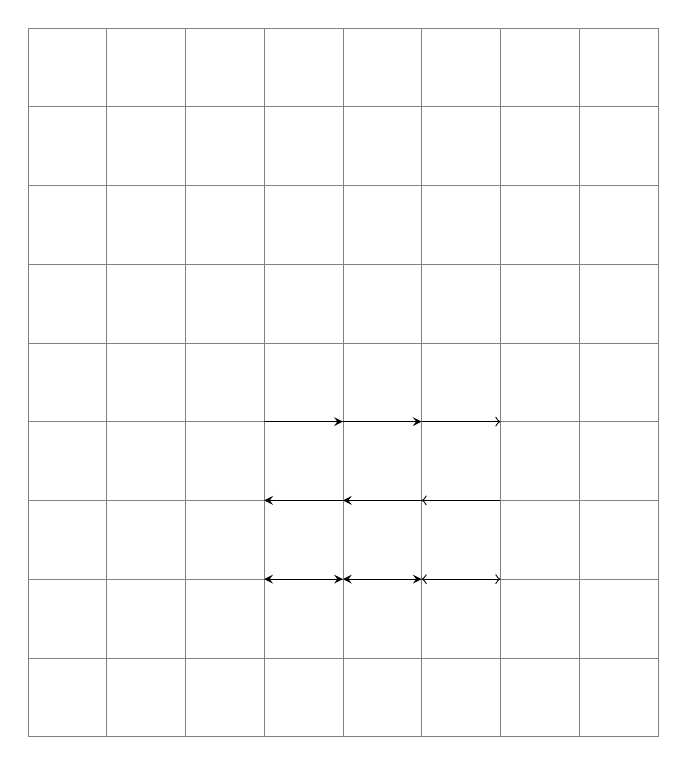
\begin{tikzpicture}

	\draw [help lines] (-3,-4) grid  (5,5);

	\draw [-stealth](0,0) -- (1,0);
	\draw [stealth-] (0,-1) -- (1,-1);
	\draw [stealth-stealth](0,-2) -- (1,-2);

	\draw [-stealth](1,0) -- +(1,0);
	\draw [stealth-](1,-1) -- +(1,0);
	\draw [stealth-stealth](1,-2) -- +(1,0);


	\draw [-to](2,0) -- +(1,0);
	\draw [to-](2,-1) -- +(1,0);
	\draw [to-to](2,-2) -- +(1,0);






\end{tikzpicture}

\end{document}
